%TÉCNICA OMNI--------------------
\chapter{TÉCNICA OMNI}
\label{chap:omni}

Neste capítulo será explanada a técnica OMNI, mencionada previamente nos Capítulos \ref{chap:introducao} e \ref{chap:conceitos}.
A técnica OMNI, sua concepção, construção e uso é retirada do trabalho de \cite{Traina2001} e \cite{Traina2007}.


\section{CONCEITOS E DEFINIÇÕES OMNI}
\label{sec:defomni}
Como apresentado anteriormente, a técnica OMNI baseia-se em em uma série de elementos chamada de 
OMNI-focos. Estes focos são elementos presentes na base de dados previamente escolhidos, e possuem como função 
servirem de marco para o cálculo das coordenadas Omni de cada elemento presente no banco.

\begin{mydef}
 \label{def:omnifoco}
 Seja um espaço métrico $M = <S,d>$, uma base de focos OMNI é um conjunto 
 $\mathscr{F} = \{f_1, f_2, ..., f_l | f_k \in S, f_k \neq f_j, l \leq N \}$ onde cada $f_k$ é um foco
 (ou ponto focal) de $S$, $l$ é o número de focos da base de focos e $N$ é o número de elementos da base de dados.
\end{mydef}

\begin {mydef}
 \label{def:omnicoord}
 Dado um objeto $s_i \in S$ e a base de focos OMNI $\mathscr{F}$, as coordenadas OMNI $C_i$ do objeto é o conjunto
 de distâncias de $s_i$ para cada foco em $\mathscr{F}$:
 \begin{equation}
  C_i = \{ <f_k, d(f_k, s_i)>, \forall f_k \in \mathscr{F} \}
 \end{equation}
\end {mydef}

Para distinguir a distância $d(f_k, s_i)$ como uma coordenada, é utilizada a notação $df_k(s_i) = d(f_k, s_i)$.\par
									
Quando um novo objeto é inserido na base de dados, as suas coordenadas OMNI são calculadas e armazenadas. Em uma pesquisa por
similaridade, estas coordenadas são utilizadas para podar o número de cálculos de distância, como ilustrado pela Figura \ref{fig:rqomni1}.\par

O custo associado a utilização da técnica OMNI provém de duas fontes: o tempo para calcular as coordenadas OMNI (cálculo da distância
entre o elemento inserido e cada um dos focos) e o espaço físico necessário para armazenar a estrutura OMNI, geralmente armazenada em disco.
Como o número de focos necessários usualmente é baixo, estes custos atrelados a técnica OMNI são menores do que o ganho
de desempenho nas consultas.

\section{USO DA BASE DE FOCOS}
Os problemas entre a escolha da base de focos $\mathscr{F}$ e a sua cardinalidade $l$ são intimamente relacionados. Quanto
mais focos, mais espaço e tempo para processamento é necessário. Por isso, é necessário maximizar o ganho de desempenho com
a menor quantidade possível de focos.

\begin{mydef}
 Dado uma base de focos OMNI $\mathscr{F} = \{f_1, f_2, ..., f_l\}$ e uma coleção de objetos $A = \{x_1,x_2,...,x_n\} \subset \mathbb{S}$, a
 região OMNI de delimitação mínima (\textit{minimum bounding OMNI region - mbOr}) de $A$ é definido como a interseção
 dos intervalos métricos $R_A = |\  ^{l}_{1}I_i$, onde $I_i = [min(d(f_i,x_j)), max(d(f_i,x_j))],\ 1\leq i \leq l,\ 1 \leq j \leq n$. 
\end{mydef}

A ideia gráfica de uma \textit{mbOr} foi previamente apresentada na Figura \ref{fig:rqomni1} para o caso de uma consulta utilizando um único foco.
É possível ver que a \textit{mbOr} sempre inclui todos os elementos do conjunto-resposta, mas pode incluir elementos que não são pertinentes
ao conjunto-resposta (alarmes falsos). Embora seja necessária mais uma etapa de cálculo de distâncias (etapa de refinamento), o número de cálculos é
reduzido drasticamente com o uso da \textit{mbOr}.\par

Uma \textit{mbOr} pode ser reduzida ainda mais com o uso de múltiplos focos, como ilustra a Figura \ref{fig:rqomni2}.

\begin{figure}[H]
\centering
\caption{Consulta por abrangência pela técnica OMNI utilizando dois focos}
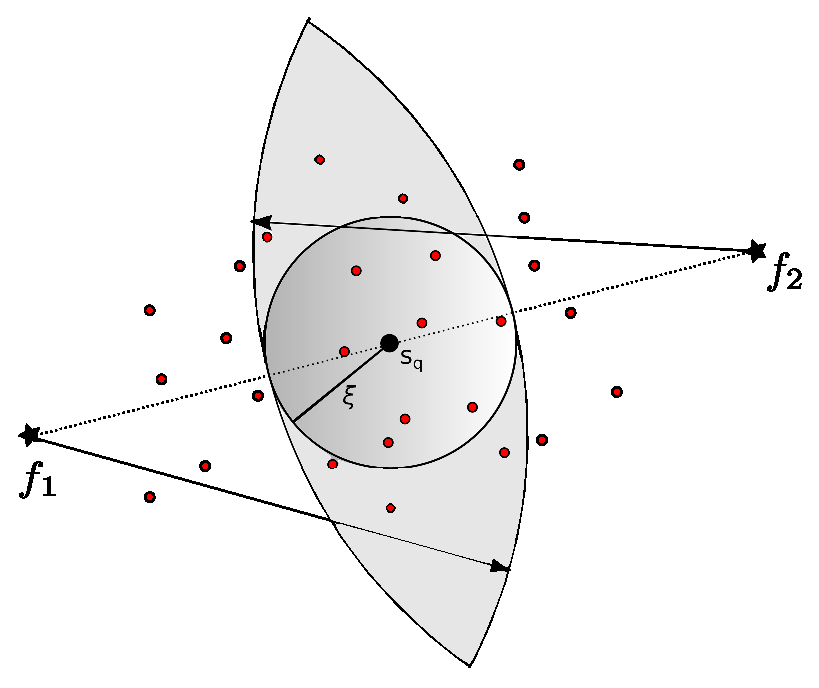
\includegraphics[width=.6\textwidth]{dados/figuras/rg_omni_2.eps}
\fonte{Autoria Própria}
\label{fig:rqomni2}
\end{figure}
								
Considerando a família Minkowski de distâncias (métricas $L_p$), um número de focos correspondente ao valor da
dimensão intrínseca da base de dados acrescido de um ($\lceil D \rceil +1$) seria o suficiente para maximizar a performance da técnica OMNI. O uso de mais focos do que o 
necessário traria pouca ou nenhuma redução à mbOr. Este valor da dimensão intrínseca pode ser obtido através da técnica de box-counting \cite{Block1990}.

\section{ESCOLHA DOS FOCOS}
\label{sec:escoco}
Para a escolha dos focos OMNI, o elemento candidato a foco deve pertencer a base de dados. Isso se deve ao fato de que algumas vezes
é impossível sintetizar um objeto de uma base de dados, como uma impressão digital. O algoritmo utilizado para o encontro dos focos
é o algoritmo HF. Esse algoritmo procura aleatoriamente um elemento $s_1$, encontra o elemento $f_1$ mais distante daquele e o seleciona como
o primeiro foco. Após isso, procura pelo elemento $f_2$ mais longe de $f_1$ e o seleciona como o segundo foco, e armazenando
a distância entre eles como $borda$.\par

O próximo foco é o elemento com as distâncias mais similares aos outros focos previamente escolhidos. Para cada objeto
$s_i$ não escolhido como foco ainda, o erro da distância em relação à borda é:
\begin{equation}
 erro_i = \sum_{k}^{k é foco} |borda - d(f_k, s_i)|
\end{equation}

\begin{algorithm}
\label{alg:hf}
    \caption{Algoritmo HF}
    \KwIn{a base de dados $\mathbb{S}$ e o número de focos $l$}
    \KwOut{base de focos OMNI $\mathscr{F}$}
    Início\\
       1.Selecione aleatoriamente um objeto $s_i \in \mathbb{S}$.\\
       2.Encontre o objeto $f_1$ mais longe de $s_i$. Insira $f_1$ em $\mathscr{F}$.\\
       3.Encontre o objeto $f_2$ mais longe de $f_1$. Insira $f_2$ em $\mathscr{F}$.\\
       4.Defina $borda=d(f_1,f_2)$, usada para calcular $erro_i$.\\
      \While{existirem focos a serem determinados}{
	  5.Para cada $s_i \in \mathbb{S},\ s_i \notin \mathscr{F}$: calcule $erro_i$.\\
	  6.Selecione $s_i \in \mathbb{S}$ de tal modo que $erro_i$ seja mínimo.\\
	  7.Insira $s_i$ em $\mathscr{F}$.
      }
\end{algorithm}

O algoritmo HF requer $l*N$ cálculos de distância. O Algoritmo \ref{alg:hf} mostra que as etapas 3 e 5 são cálculos
necessários para a determinação das coordenadas OMNI de cada objeto. Isso mostra que o algoritmo HF também prepara as
coordenadas OMNI da base de dados. Outro fato importante é o da base de focos OMNI ser invariável a operações de inserção
ou remoção na base.

\section{INDEXAÇÃO DAS COORDENADAS OMNI}
\label{sec:indexomni}

Objetos em um espaço métrico não são ordenáveis, portanto métodos de acesso baseados na propriedade de ordenação total
como B-Trees não podem ser utilizados diretamente para a sua indexação. No entanto, as distâncias $df_k(s_i)$ de cada foco
$f$ para a base de objetos pode ser ordenada e indexada por estruturas B-Tree. Assim, é possível armazenar as coordenadas OMNI
em um conjunto de $h$ B-Trees, sendo $h$ o número de focos da base. Cada nó da \textit{k-ésima} B-Tree é composto pela distância $df_k(s_i)$
e o identificador interno do objeto \textit{IOid}($s_i$). Este conjunto de B-Trees é chamado de OMNIB-Forest, e fornece 
um suporte efetivo para bases de dados imersas em um espaço métrico, utilizando recursos nativos a SGBDRs.\par

Um exemplo do uso das coordenadas OMNI para a filtragem inicial do cálculo de distância dos objetos da base em relação ao elemento central da consulta no caso de uma consulta por
abrangência pode ser visto abaixo.

\begin{figure}[H]
\centering
\caption{Base de elementos de exemplo para uma consulta por abrangência utilizando um foco}
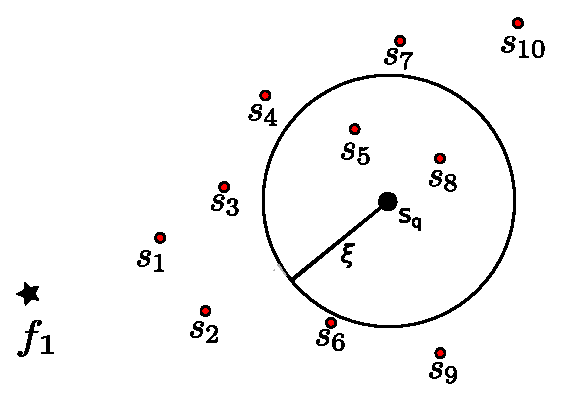
\includegraphics[width=.55\textwidth]{dados/figuras/rg_ex1.eps}
\fonte{Autoria Própria}
\label{fig:rgex1}
\end{figure}

A Figura \ref{fig:btree} representa a OMNIB-Tree utilizada para armazenar as coordenadas OMNI dos objetos da base em relação ao foco $f_1$. Nela foram armazenadas
a distância do objeto $s_i$ até o foco, e um identificador do objeto.

\begin{figure}[H]
\centering
\caption{OMNIB-Tree utilizada para o exemplo}
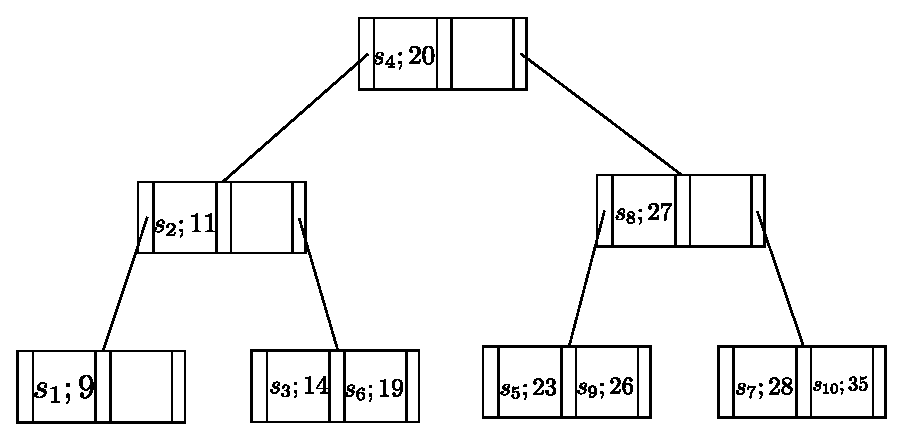
\includegraphics[width=.8\textwidth]{dados/figuras/btree.eps}
\fonte{Autoria Própria}
\label{fig:btree}
\end{figure}

A partir de uma análise geométrica, é possível perceber que um elemento candidato a estar presente no conjunto de resposta deve ter a sua distância em relação ao foco maior ou igual a distância do elemento central de consulta menos o valor do
raio da consulta, formando, assim, um limite inferior. Analogamente, o limite superior pode ser definido utilizando a distância do elemento central da consulta até o foco mais o valor do raio da consulta.

\begin{equation} \label{eq:omnirq}
|d(f_k, s_q) - \xi| \leq d(f_k, s_i) \leq |d(f_k, s_q) + \xi|
\end{equation}

\begin{figure}[H]
\centering
\caption{Análise geométrica dos limites dos elementos candidatos}
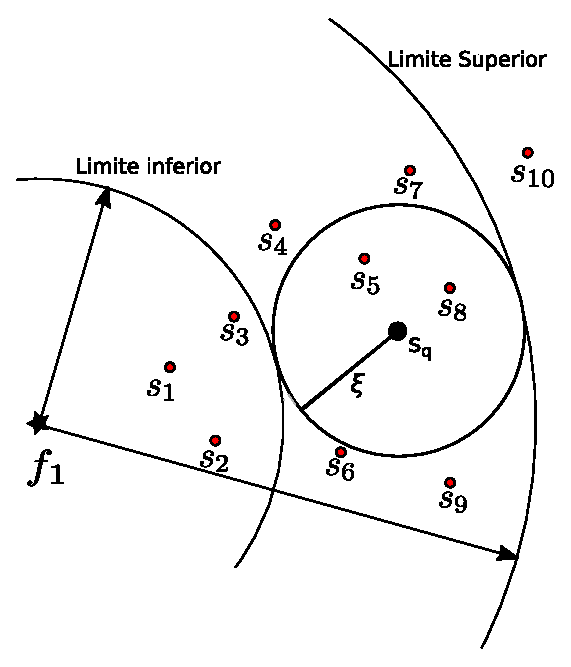
\includegraphics[width=.55\textwidth]{dados/figuras/rg_ex2.eps}
\fonte{Autoria Própria}
\label{fig:rgex2}
\end{figure}
A Figura \ref{fig:rgex2} ilustra a utilização da propriedade da desigualdade triangular para a etapa de filtragem. Tomando o elemento $s_3$ como referência e a equação da desigualdade triangular apresentada
na Definição \ref{def:espmet}, é possível definir que:
\begin{equation} \label{eq:omnirq2}
d_{f_1}(s_3) \leq d_{f_1}(s_q) + d(s_3, s_q)
\end{equation}
\begin{equation} \label{eq:omnirq3}
d(s_3, s_q) \geq |d_{f_1}(s_3) - d_{f_1}(s_q)|
\end{equation}\par
Utilizando o conceito de bola apresentado pela Definição \ref{def:bola}, se o elemento $s_3$ só pode pertencer a bola de consulta se a distância
$d(s_3, s_q)$ for menor do que o raio de consulta $\xi$. Com a Equação \ref{eq:omnirq3}, é possível definir que o elemento está fora do conjunto
de elementos candidatos se:
\begin{equation} \label{eq:rqtri}
 |d_{f_1}(s_3) - d_{f_1}(s_q)| \geq \xi
\end{equation}\par
Sabendo que a distância $df_1(s_q)$ é de 23 unidades e o raio da consulta por abrangência é de 8 unidades, utilizando a Equação \ref{eq:omnirq} é possível determinar que a distância $d(f_k, s_i)$ do elemento candidato precisa ser $\geq 15$ e $\leq 31$.
Utilizando a OMNIB-Tree criada para o foco $f_1$, é possível encontrar os elementos candidatos que prosseguirão para a etapa de refinamento, sendo eles: $s_4, s_5, s_6, s_7, s_8, s_9$. É possível notar que estes candidatos estão em conformidade com o que
foi previsto utilizando uma análise geométrica fornecida pela Figura \ref{fig:rgex2}. Também é possível verificar a validade da Equação
\ref{eq:rqtri}, pois esta fornece o mesmo conjunto de elementos encontrados com a análise geométrica.\par

É importante notar que nem todos os elementos selecionados durante a etapa de filtragem da técnica OMNI pertencem ao conjunto resposta. Na \textit{mbOr}, pode ocorrer a presença
de elementos que não estão dentro da bola da consulta por abrangência (alarmes falsos). Para minimizar o número de alarmes falsos, múltiplos focos podem ser utilizados, como demonstrado pela Figura \ref{fig:rgex3}.
Para este exemplo, o elemento $s_{10}$ é escolhido como um novo foco $f_2$. O elemento $s_6$ é descartado antes da etapa de refinamento, o que não acontece para uma filtragem utilizando um único foco.

\begin{figure}[H]
\centering
\caption{Etapa de filtragem com dois focos}
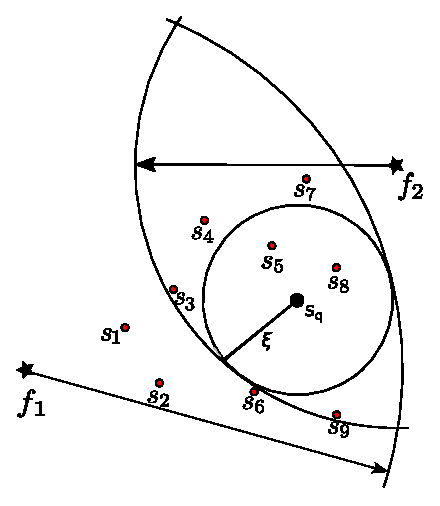
\includegraphics[width=.55\textwidth]{dados/figuras/rg_ex3.eps}
\fonte{Autoria Própria}
\label{fig:rgex3}
\end{figure}


